\chapter[2022 May]{May 2022}

\section[2022/05/07]{Friday, 06 May 2022}

\subsection{Libfreenect library installation}

Multiple hours were spent attempting to install the necessary libraries to enable communication with the Microsoft Kinect camera and the Macbook Air M1. The principle problem appeared to be installing the C-compiled libfreenect library into a useable Python module that could be installed into the virtual "kinect-project" anaconda environment being used for the prototyping. The libfreenect library first had to be compiled and built locally - which was achieved after modifying a few settings but then had to be installed by running a setup.py file to incorporate these C files into a Python wrapper module that could be used from other Python code. This installation failed nearly one hundred times as it could not find the requisite C libraries on the filesystem. After much trial and error, the installation eventually succeeded and the libfreenect library was made available for interfacing with a Kinect connected to the laptop. The successful import of the libfreenect library in a Python file on the laptop is visible in \FigRef{fig:libfreenect_success}.

\begin{figure}[h]
    \centering
    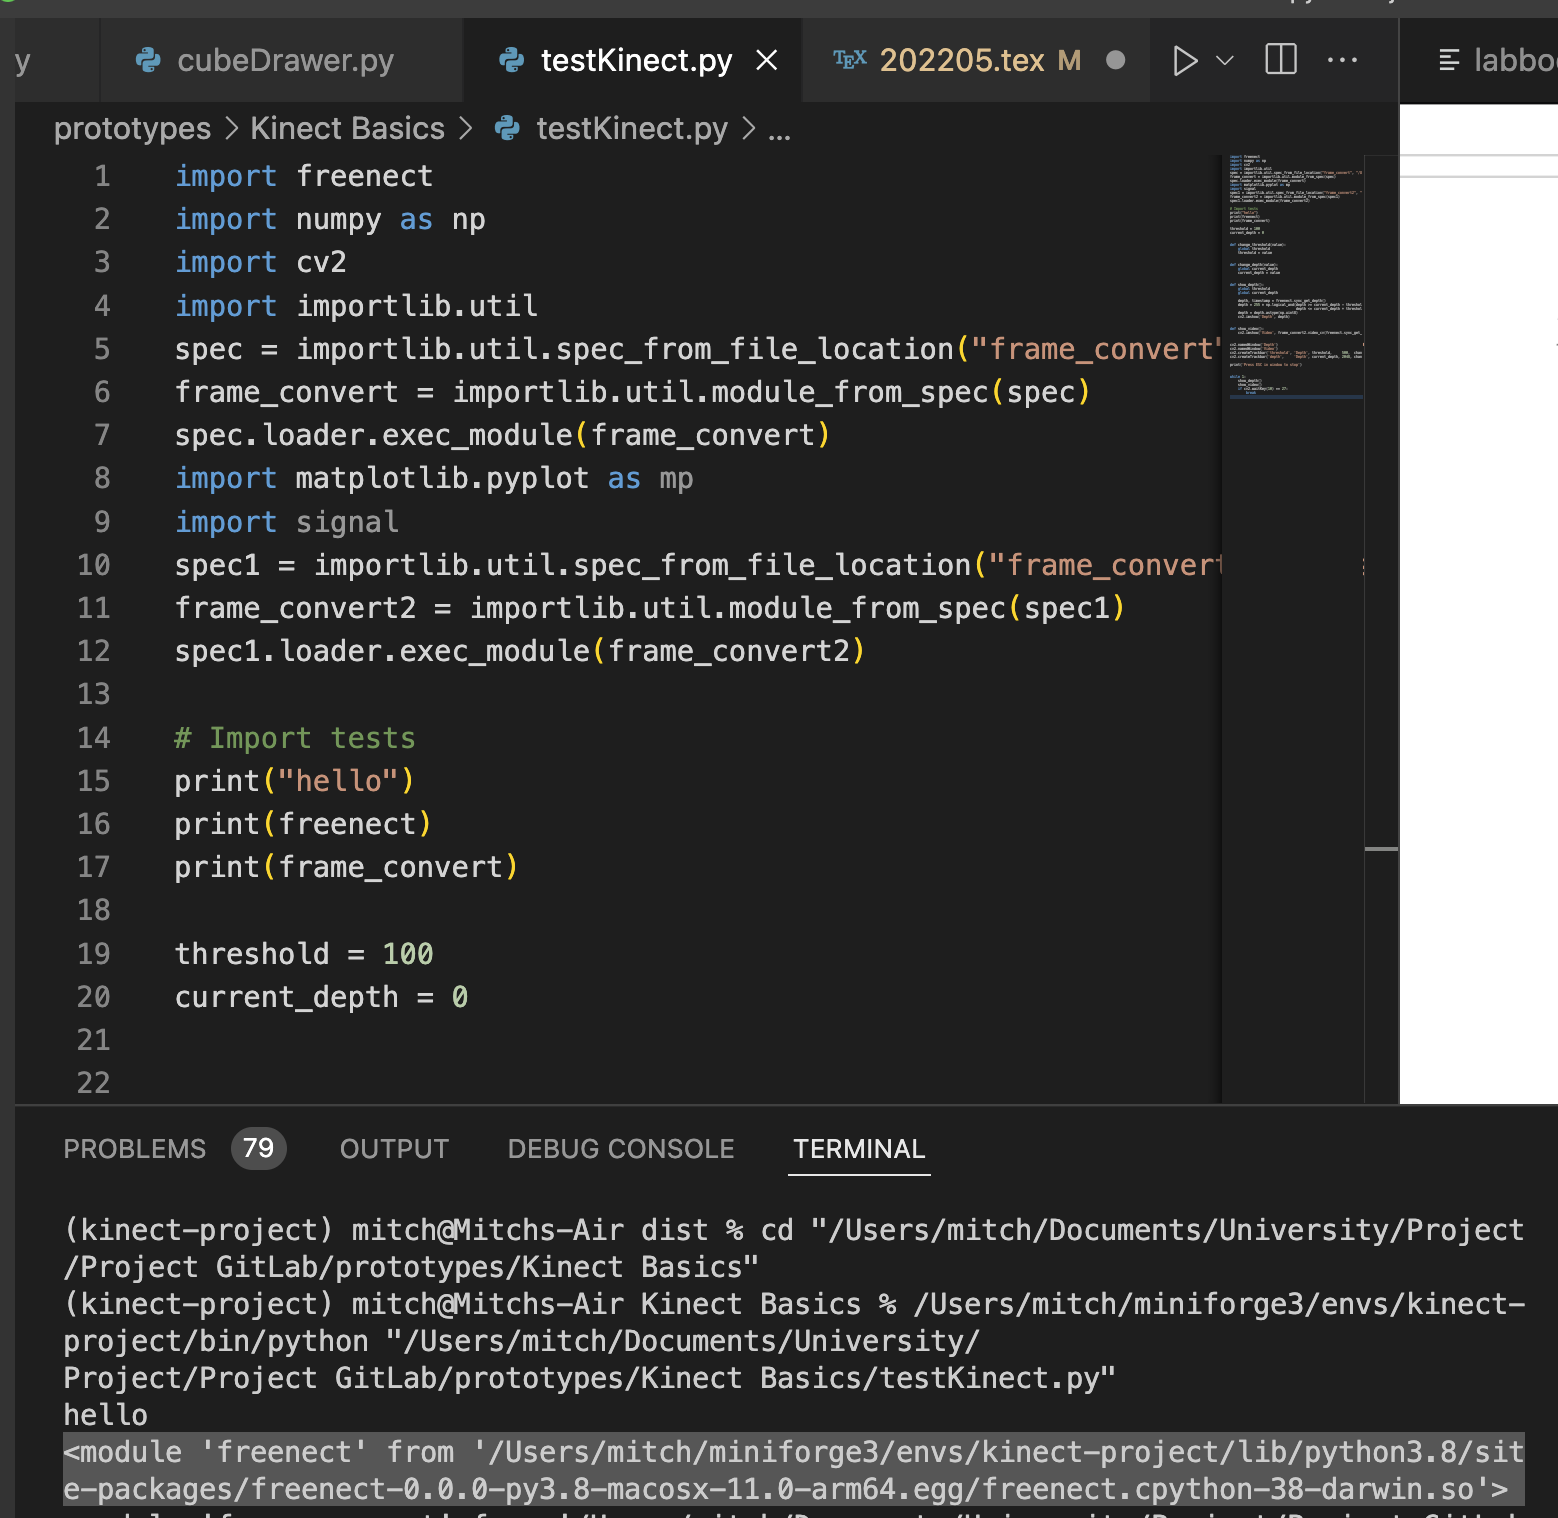
\includegraphics[width=0.5\linewidth]{figures/libfreenect_success.png}
    \caption{Successful output of importing the libfreenect library}
    \label{fig:libfreenect_success}
\end{figure}

The steps to connect the Kinect to the laptop and successfully interact with it in Python code are as follows.

\begin{itemize}
    \item Plug in Kinect to power and USB
    \item Run in Kinect-project conda environment
    \item If can't claim USB error occurs - run sudo freenect-glview first
    \item Run kinectBasics.py or other file with libfreenect commands in it
\end{itemize}

\section[2022/05/07]{Saturday, 07 May 2022}

\subsection{Virtual object control prototype using gesture input}

The objection of this session is to construct a barebones prototype that can control a virtual object using gesture control. \\

The \href{https://mediapipe.dev}{mediapipe} hands system is a freely available and excellent hand skeleton recognition system built to take camera input and output a 21-landmark hand model in realtime. This will be utilized as an off-the-shelf solution at first for part of the gesture recognition system. A CDN version of the model is available online and this is integrated into a local HTML, CSS and Javascript project so that a laptop camera can be used for input to the prototype. The prototype HTML file and CDN model can only run on a webserver and not just by opening the HTML file in a browser thus the WebServer For Chrome extension was used to run a local web server to host the application. Code was repurposed from the official mediapipe hands demo program available online. \FigRef{fig:mediapipe_app} shows the prototype application running on a laptop. 

\begin{figure}[h]
    \centering
    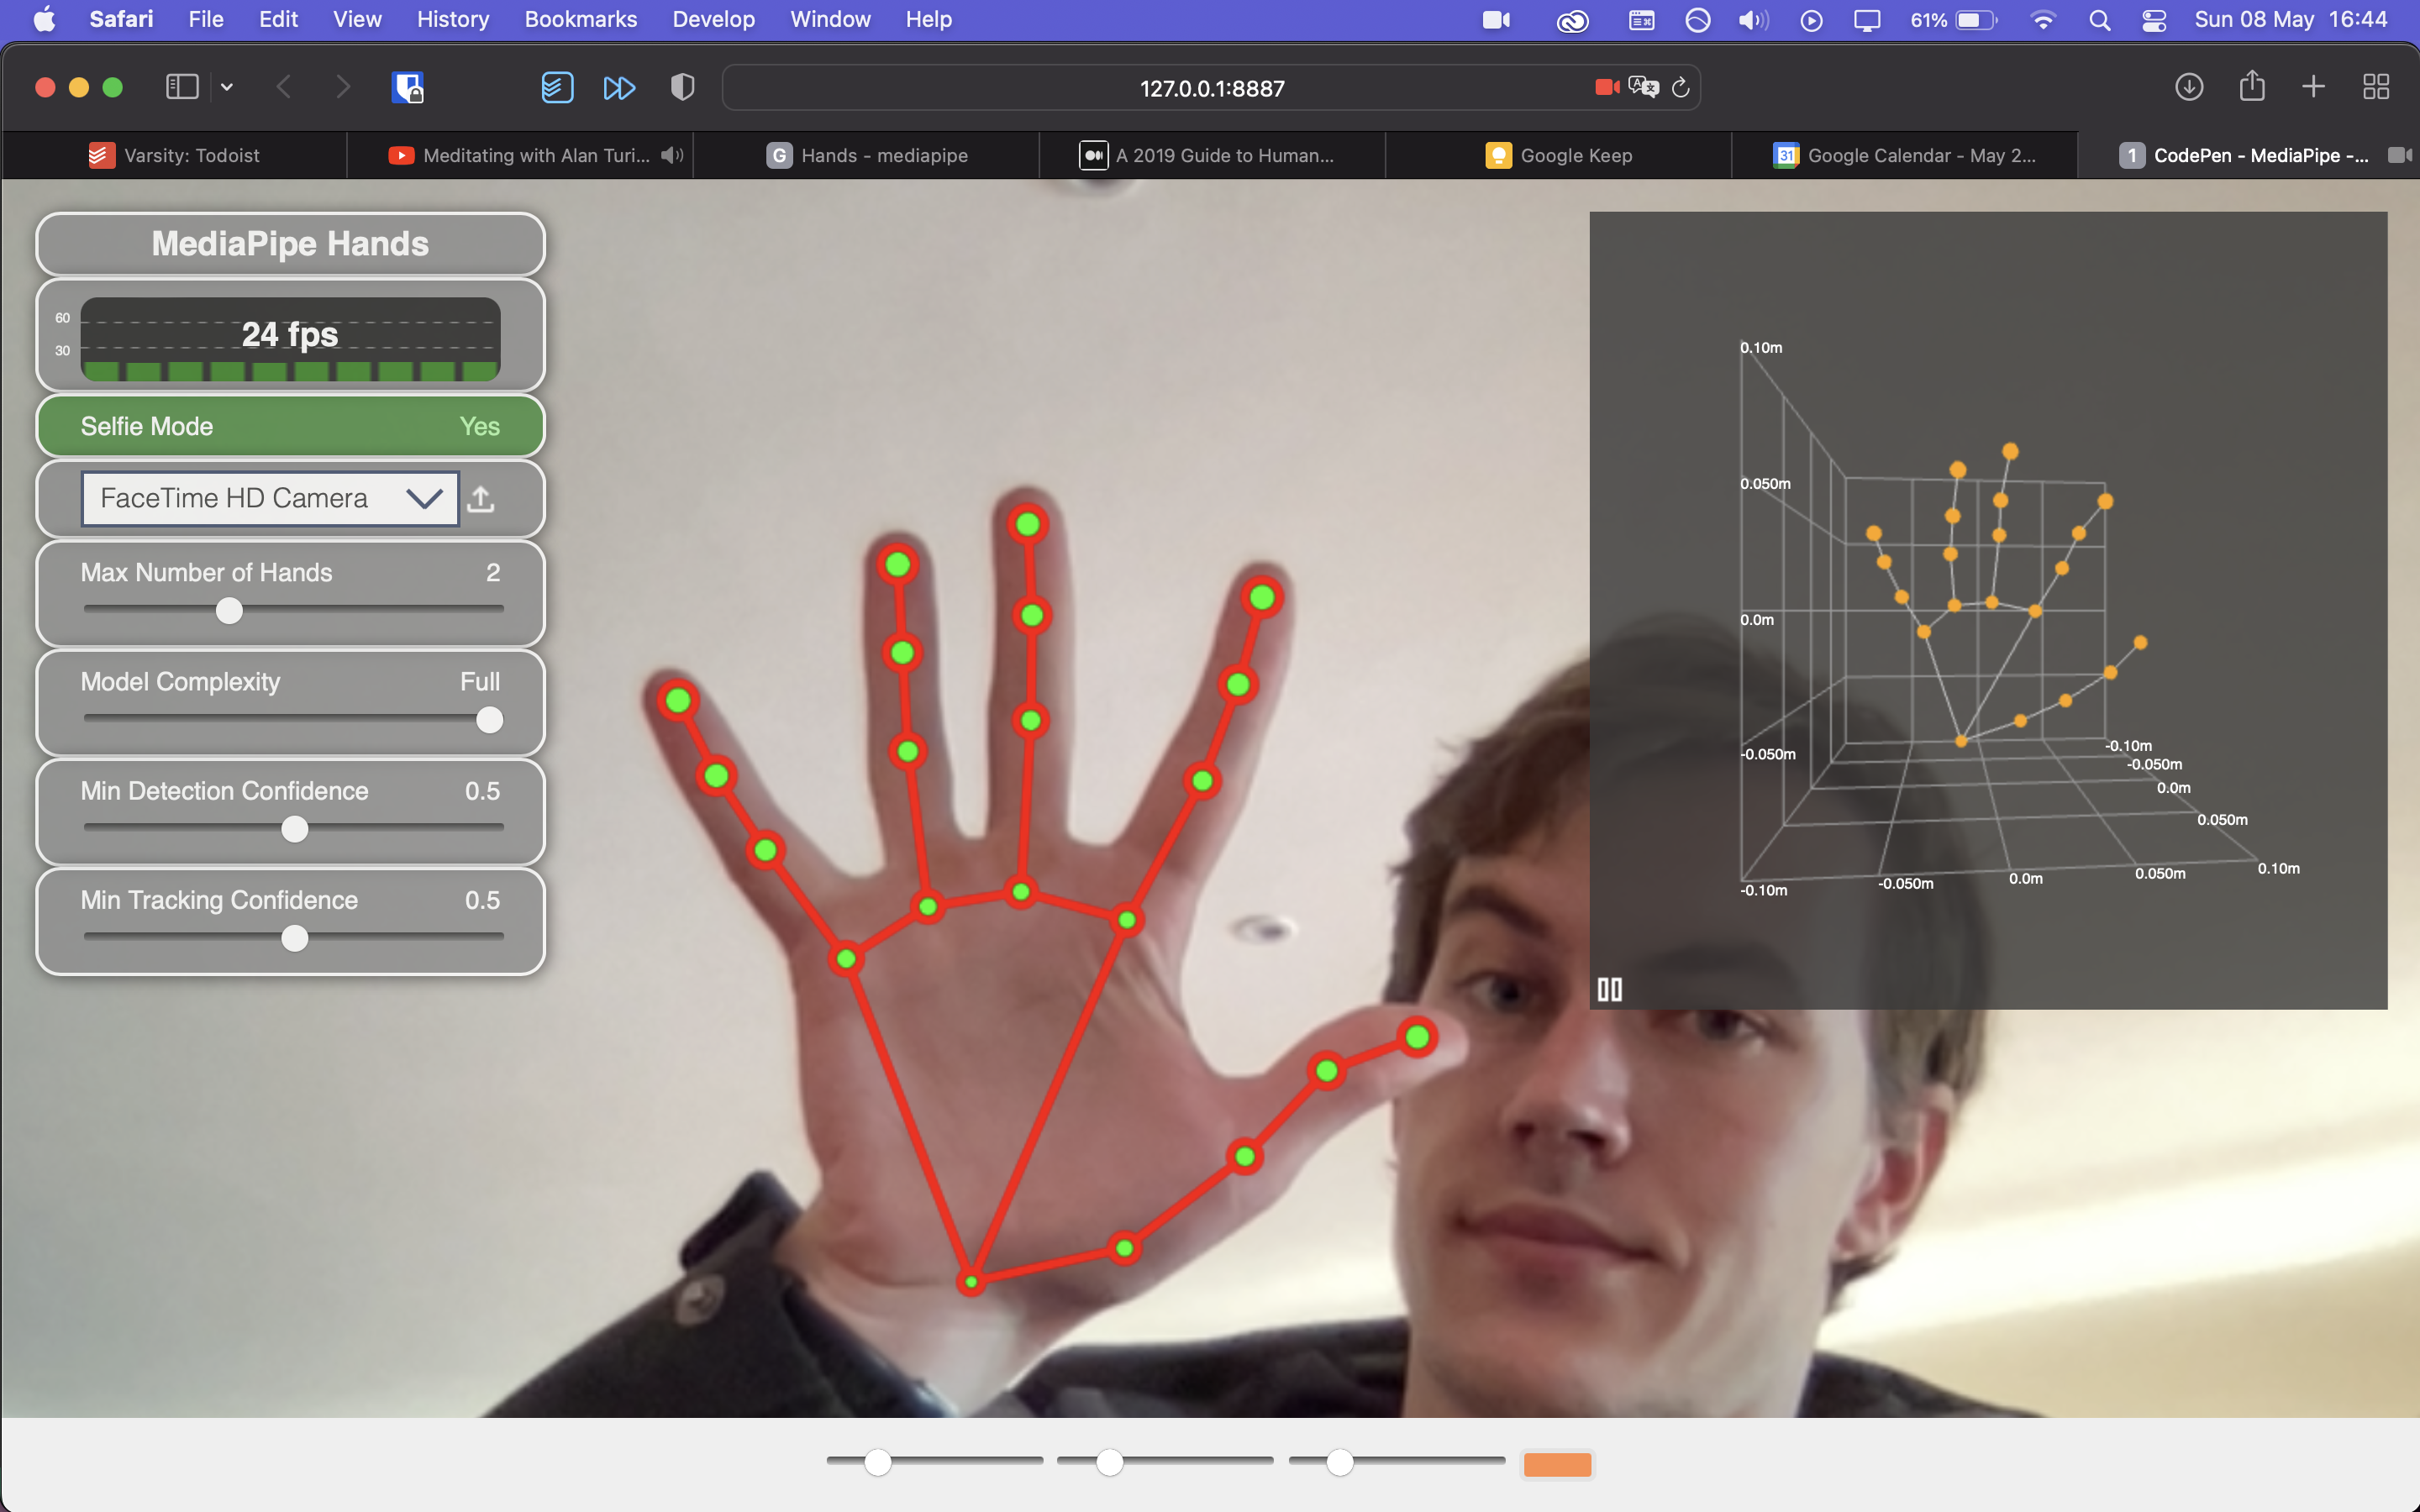
\includegraphics[width=0.7\linewidth]{figures/mediapipe_app.png}
    \caption{Local mediapipe hand model prototype}
    \label{fig:mediapipe_app}
\end{figure}

Mediapipe was not available for Python for the laptop being used for the prototype but the Kinect library available was only available in Python. In order to interface the mediapipe implementation with the Kinect a way of connecting a Javascript and Python program was necessary. To that end, a Python Flask web server was created in a separate Python file to receive information from the hand model. This Flask implementation waited for a PUT request on port 5000 and the Javascript app was set up to send the information for landmark[20] over this connection - the x,y and z co-ordinates for the pinky finger. This was received by the Flask app and then written to a text file. A third program was created in Python to read the values from the text file and draw a cube at co-ordinates matching those of the latest gesture interpretation of the pinky finger over a static image - to be replaced by the feed from the Kinect at a later stage. \\

The result of this system is presented in \FigRef{fig:mediapipe_prototype_output} and shows how moving the user's hand renders the cube in different locations over the image. Because of the multiple files being used to hack together this prototype it runs very slowly and the output is extremely laggy compared to hand input. However, the proof of concept is shown - a virtual object can be manipulated simply by tracking the position of one of the user's fingers using a webcam as input. Aspects to consider for the fully-fledged implementation from first principles are connecting the system to a depth-sensing camera for depth information of the environment, reducing the number of memory storage and retrieval operations between accepting input data from the hand model and cube rendering steps as well as mapping the hand model input to control of the virtual object better than just tracking a single finger - how the hand moves and how fast should also influence the output imagery. \\ 

\begin{figure}[h]
    \centering
    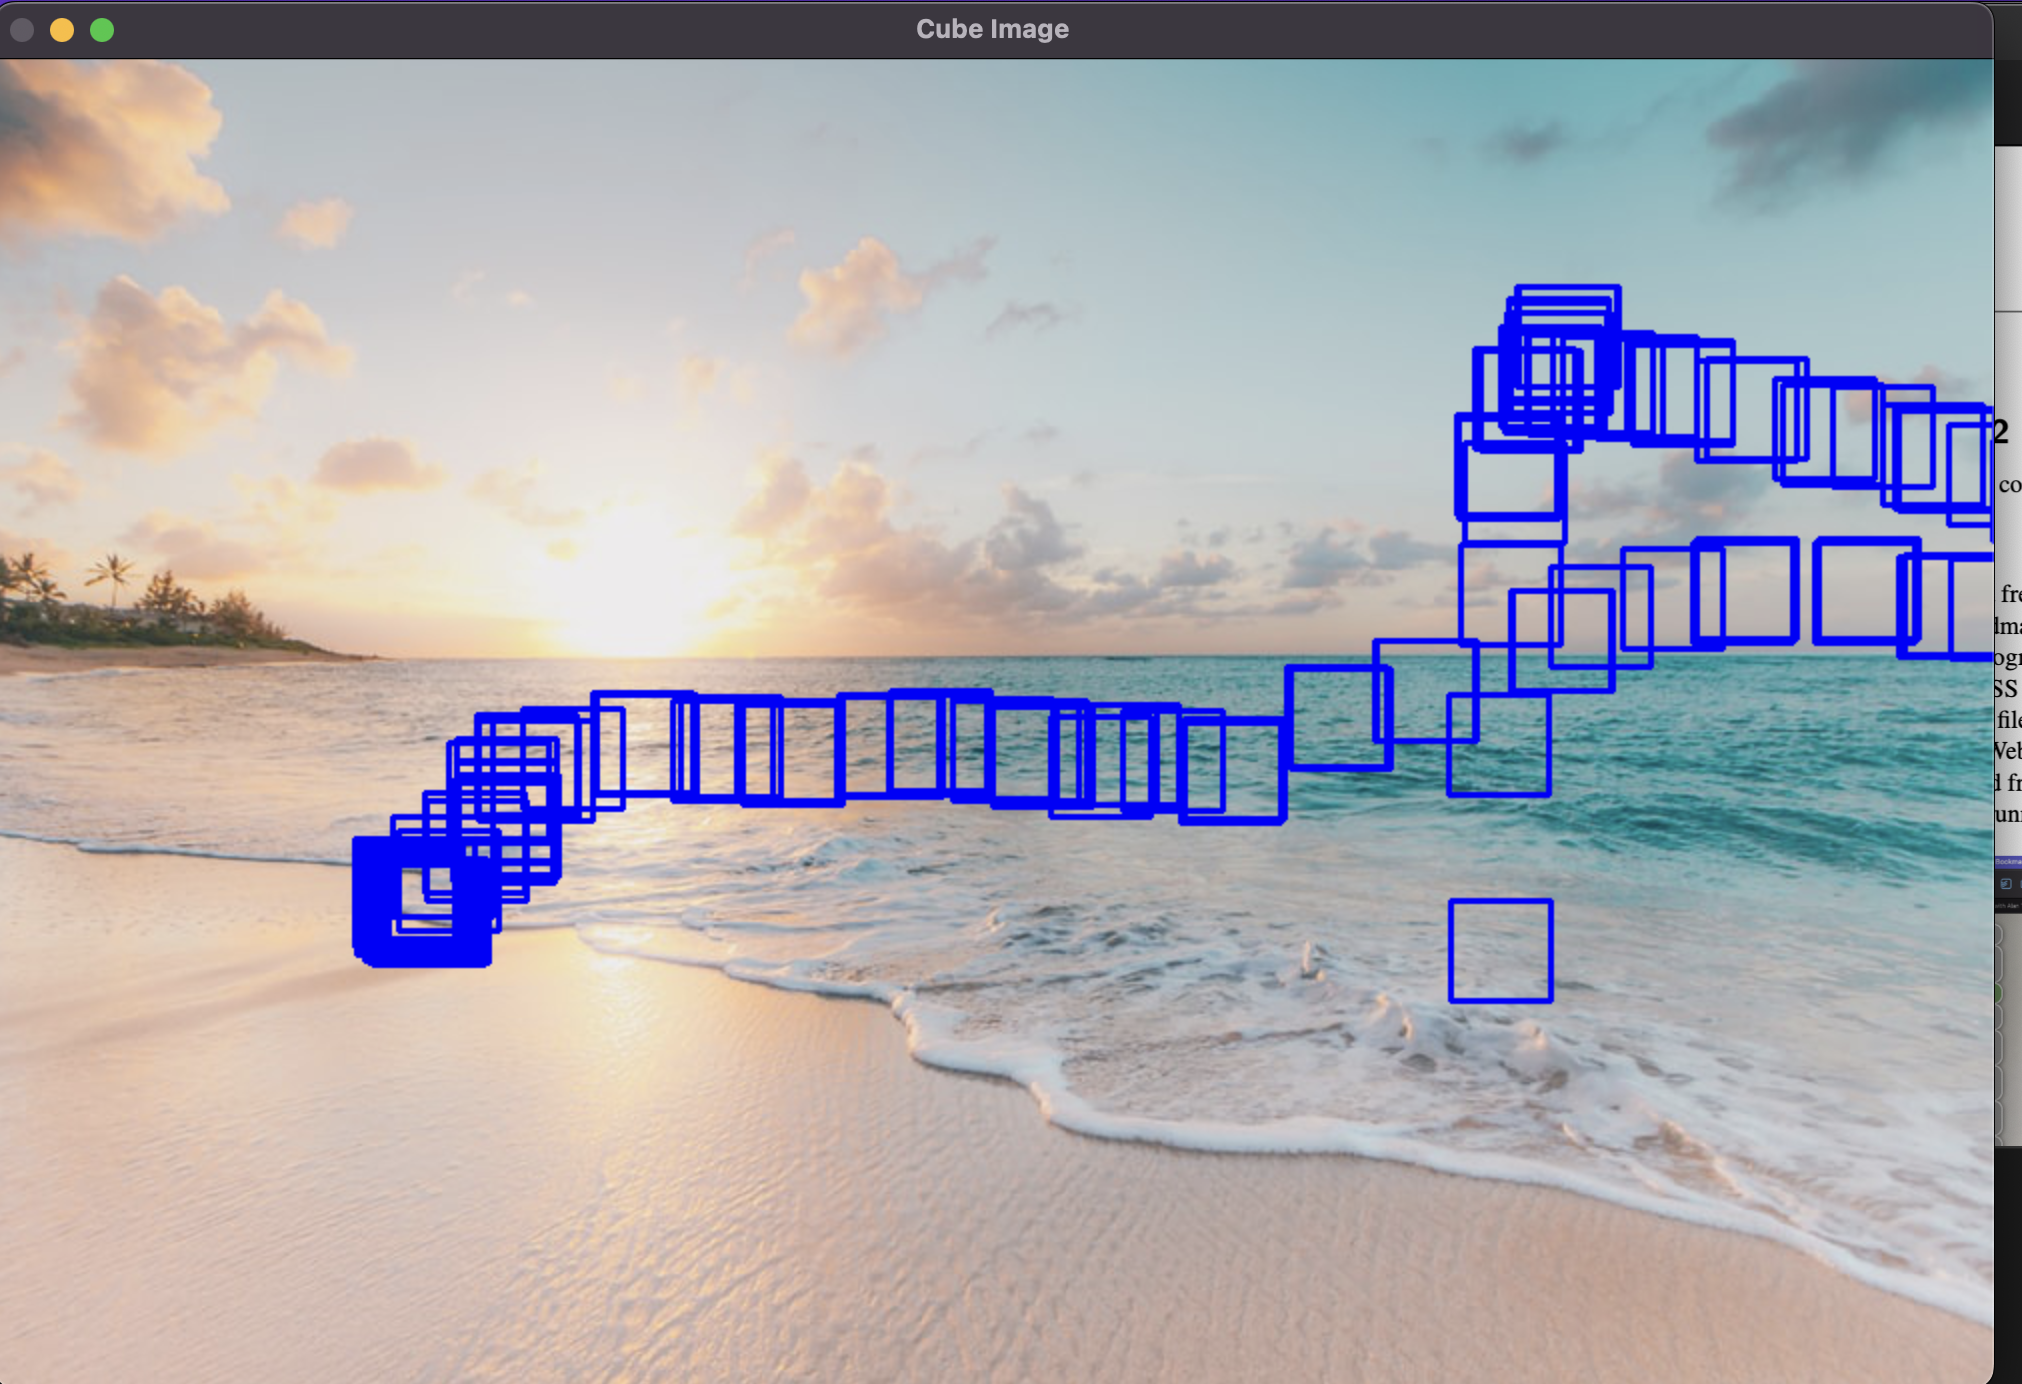
\includegraphics[width=0.7\linewidth]{figures/mediapipe_prototype_output.png}
    \caption{Output of mediapipe hand model prototype}
    \label{fig:mediapipe_prototype_output}
\end{figure}

In order to run the various files together to get the prototype functioning correctly the following instructions have to be followed. 
\begin{itemize}
    \item Start Chrome web server in dist folder of media pipe folder
    \item Run flask.py program
    \item Open index.html of mediapipe folder
    \item Run cubeRunner.py program
    \item Move hands in desired manner
\end{itemize}

\section[2022/05/09]{Monday, 09 May 2022}

\subsection{Joint regression research}

Research was conducted on how the industry standard approach to pose estimation works - the broad subfield that hand gesture recognition falls into. A \href{https://heartbeat.comet.ml/a-2019-guide-to-human-pose-estimation-c10b79b64b73#0057}{summary} of pose estimation research papers from various institutions points to the general trend of convolutional neural networks being used for linear joint regression - in which the location of particular human joints in various images is slowly learned from labelled data. In particular, the Deep Pose implementation \cite{deep_pose} by Toshev et al. uses this approach to great success by stacking a number of layers after each other, alternating whether the layer is a linear or non-linear transformation in a general Deep Neural Network (DNN) model. More research into the details of convolutional neural networks, activation functions and transformations that work well with image data is needed.\\ 

\section[2022/05/16]{Monday, 16 May 2022}

The aim of this session is to elucidate the work done on developing a basic neural network in the past few days in addition to experimentation with a PC webcam as input.

\subsection{Webcam resolution prototype}

The webcam of a modern PC is accessible by Python libraries and can be used as input for various programs such as the neural network developed below. Modifying the input resolution of the image is going to be a necessary step in order to train the neural network in a reasonable amount of time and thus a webcam\_resolution.py prototype was developed in order to change the resolution of a webcam from which a Python program accepts input. The front-facing webcam on a Macbook Air M1 only allows the resolutions of 1280x720px or 640x480px to be set as the input resolutions. The use of this built-in webcam versus an external piece of hardware will need to be investigated during the training process to see if larger images are too computationally intensive to train and predict with in an online fashion - without extensive preprocessing before training commences.

\subsection{Neural network prototype}

In most of the pose estimation \cite{deep_pose} and gesture recognition research papers \cite{mediapipe_hands} observed so far the solution ultimately boils down to a fully-connected neural network at the end of the processing pipeline. This is often a convolutional neural network with multiple convolution layers at the start of the network that modify an input image in various ways and then is attached to a fully-connected network at the end, which learns complex patterns in the input image. Thus, the first-principles development of a neural network that can accept various size inputs and train effectively is a necessity for this project. \\

To that end, the NN.py prototype was constructed which has one input layer, one hidden layer and one output layer of two neurons each. An array of hidden layer biases and output layer biases are also present. These values are easily modifiable to be larger later. The activation function used to activate each neuron after the weighted inputs have been summed is the sigmoid function because of its easily calculable derivative. This too can be changed out for a RELU or tanh function later should the system require it.\\

The backpropagation algorithm is implemented in the standard method of calculating errors at the output layer based on expected output for a given input, working out the delta values required to modify each output neuron to its expected value and then methodically working backwards through the network to calculate the error and delta at each neuron based on the errors and deltas further forward in the network. The weights between layers are then updated using the delta values, learning rate and input values to that weight. This is done successively for multiple input training data items and the whole process is repeated for a number of epochs in order to train the network successfully. \FigRef{fig:NN_input_graph} shows the rough distribution of the training data and how the neural network needs to learn to differentiate between the two different groups of points. The results of the training process are visible in \FigRef{fig:NN_prototype_600_epochs} for 600 epochs and the ability of the network to learn is clearly demonstrated.

\begin{figure}[h]
    \centering
    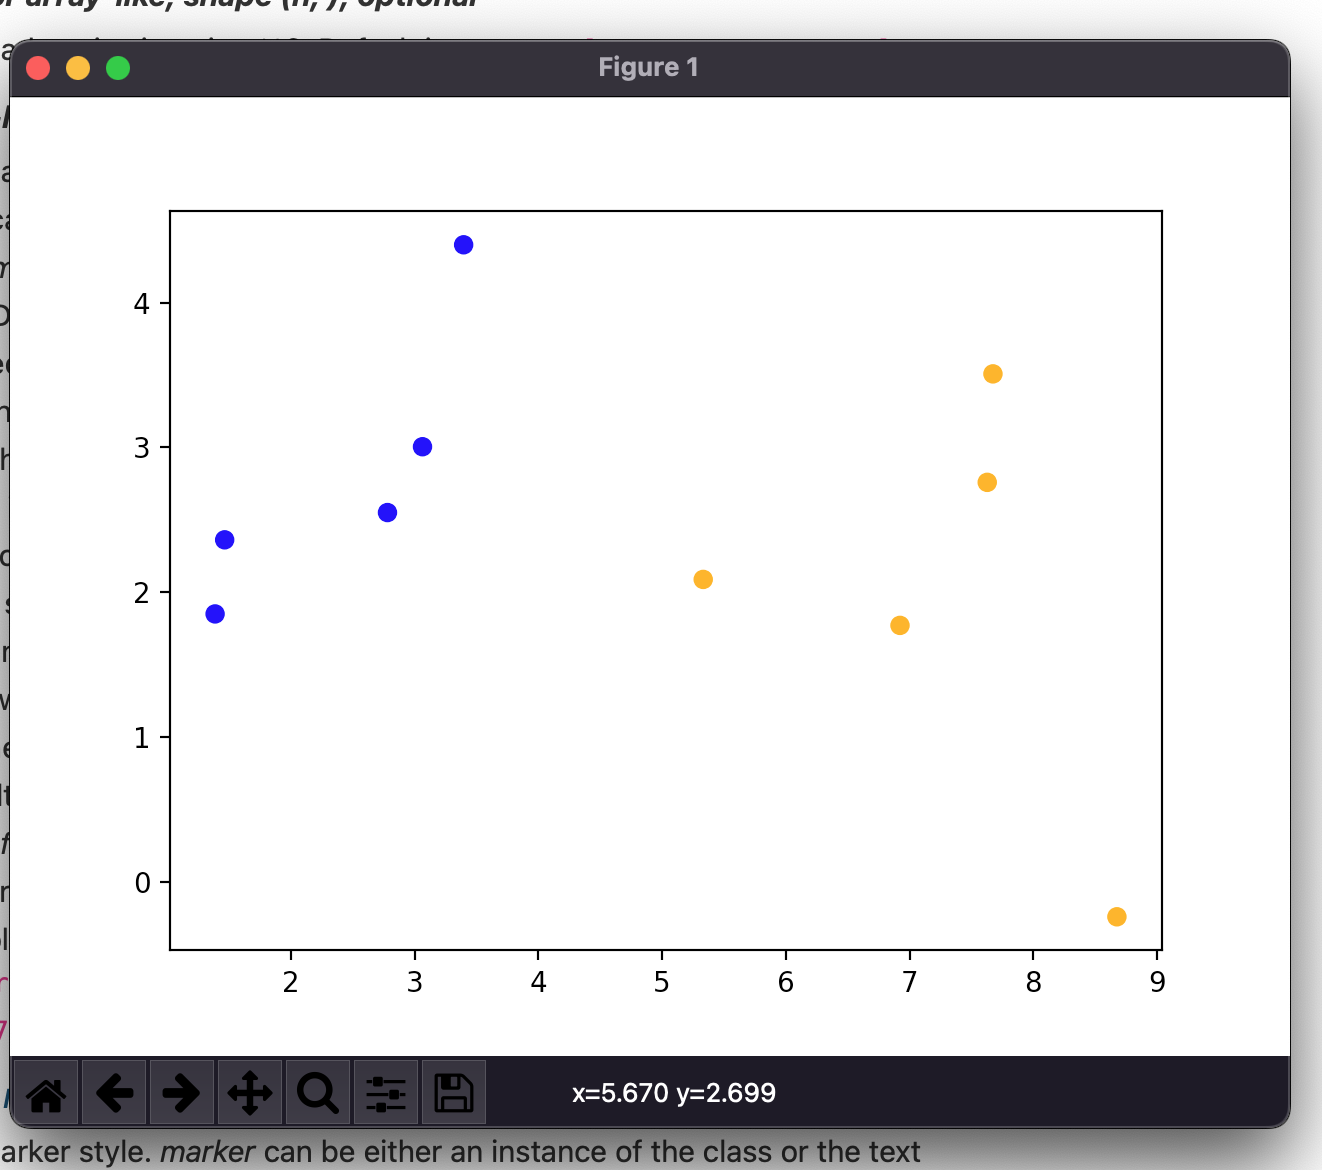
\includegraphics[width=0.5\linewidth]{figures/NN_input_graph.png}
    \caption{NN training data distribution}
    \label{fig:NN_input_graph}
\end{figure}

\begin{figure}[h]
    \centering
    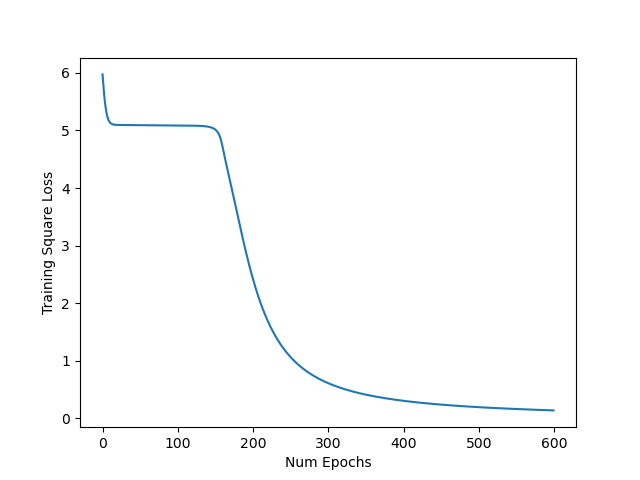
\includegraphics[width=0.6\linewidth]{figures/NN_prototype_600_epochs.png}
    \caption{NN prototype loss curve over 600 training epochs}
    \label{fig:NN_prototype_600_epochs}
\end{figure}

Similarly in \FigRef{fig:NN_prototype_10000_epochs} the use of more training epochs trains the network more rigorously and allows a lower error rate on testing data. Of note is that the network has only been tested thus far on the same training data it was originally trained with - thus extreme overfitting is no doubt occurring and techniques such as early stopping, regularization and slower learning rates will need to be investigated when training the network for complex tasks like joint regression.

\begin{figure}[h]
    \centering
    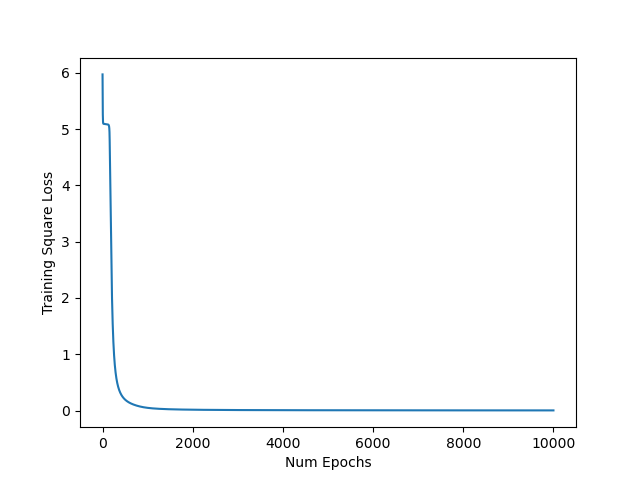
\includegraphics[width=0.6\linewidth]{figures/NN_prototype_10000_epochs.png}
    \caption{NN prototype loss curve over 10000 training epochs}
    \label{fig:NN_prototype_10000_epochs}
\end{figure}

\FigRef{fig:NN_prototype_lrate_0.1_600_epochs} shows the output of the first several epochs of training the network using a learning rate of 0.1 and clearly demonstrates the decreasing loss function as the network generalizes to the data given to it. As the epochs increase, the loss becomes even smaller and eventually reaches near-zero values and this is visible in \FigRef{fig:NN_prototype_lrate_0.1_600_epochs_end}.

\begin{figure}[h]
    \centering
    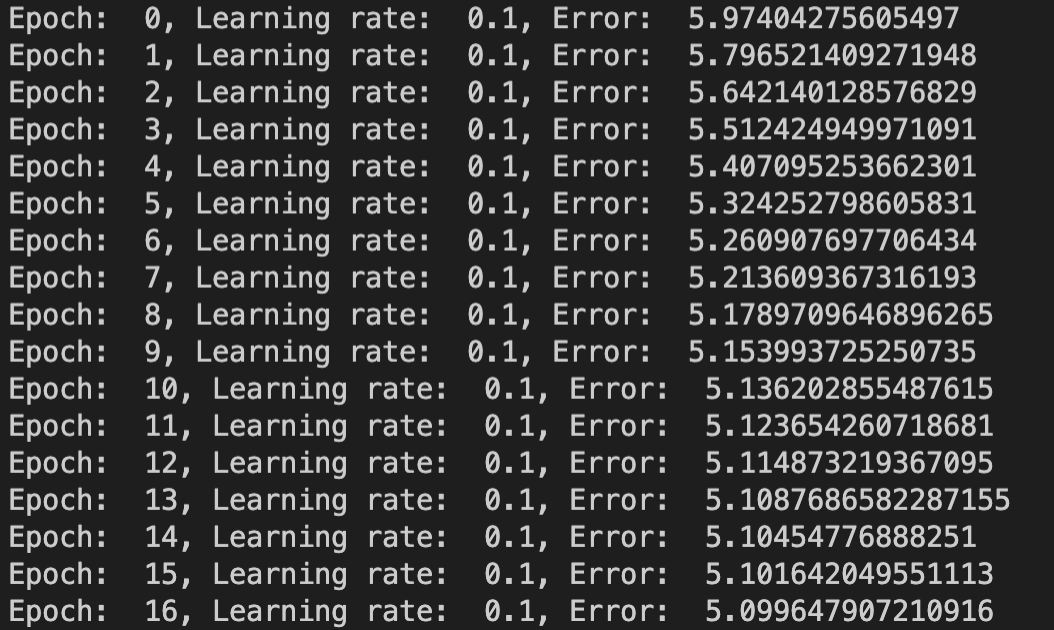
\includegraphics[width=0.7\linewidth]{figures/NN_prototype_lrate_0.1_600_epochs.png}
    \caption{NN prototype training output over 600 training epochs with learning rate of 0.1}
    \label{fig:NN_prototype_lrate_0.1_600_epochs}
\end{figure}

\begin{figure}[h]
    \centering
    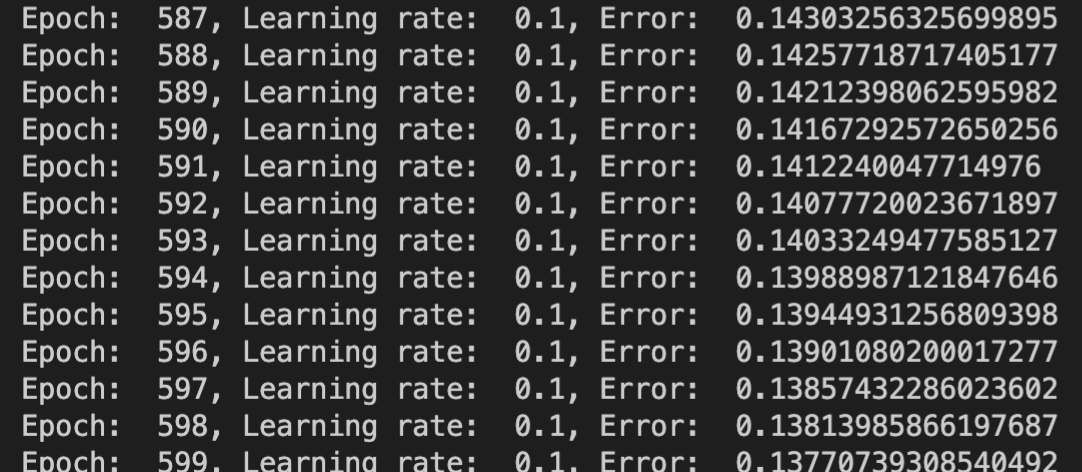
\includegraphics[width=0.7\linewidth]{figures/NN_prototype_lrate_0.1_600_epochs_end.png}
    \caption{NN prototype training output end over 600 training epochs with learning rate of 0.1}
    \label{fig:NN_prototype_lrate_0.1_600_epochs_end}
\end{figure}

\FigRef{fig:NN_prototype_overfitting_test} shows the output of a testing regime that predicts the values for all the training data inputs and achieves a 100\% accuracy for the testing.

\begin{figure}[h]
    \centering
    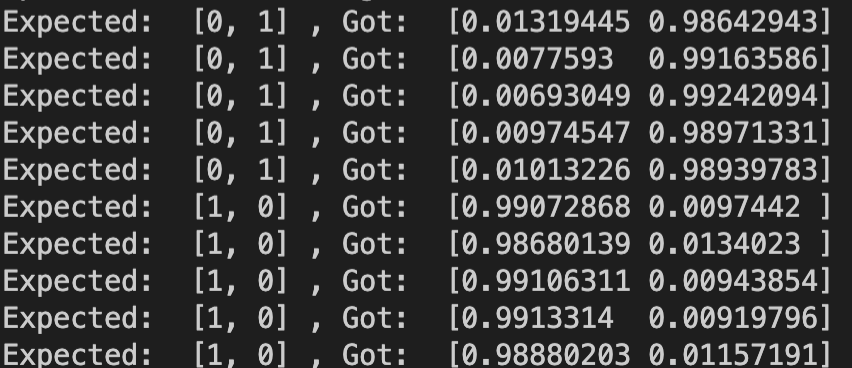
\includegraphics[width=0.7\linewidth]{figures/NN_prototype_overfitting_test.png}
    \caption{NN output of overfitting test on small input dataset}
    \label{fig:NN_prototype_overfitting_test}
\end{figure}

\section[2022/05/17]{Tuesday, 17 May 2022}

\subsection{Kernel Functions Experimentation}

The aim of this session is to investigate the purpose and ease of using kernel functions in convolutional networks.


In the research papers studied so far the use of convolutional neural networks is prevalent for taking image input and acquiring a desirable output result using a neural network. The use of these convolution layers involves multiplying the input image pixel values with various kernel functions that modify the output of the image in such a way to generalize certain regions of an image and capture nonlinear components present in the image. These kernel functions can be applied in numerous ways, including to individual RGB layers, to sums of the layers and to different parts of the image. A kernel function prototype was built in order to attempt to use these kernel functions on input images and acquire a sense of the function they perform and how they assist in a convolutional neural network's learning. \\

\FigRef{fig:kernel_identity} shows the input image that is passed into the various kernel functions. The first kernel is the edge detection 1 kernel and is presented in \FigRef{fig:kernel_edge_detection_1}. The rough edges of the person in the input image are visible using this kernel. A more prominent and striking interpretation of the edges of the image's content is visible in \FigRef{fig:kernel_edge_detection_2}. Two alternative kernel functions are presented in the Left and Right Sobel kernel functions respectively in \FigRef{fig:kernel_left_sobel} and \FigRef{fig:kernel_right_sobel}. The utility of these kernel functions is apparent in that they extract meaningful information from an input image and allow reduced computation to occur in a neural network while still representing salient features of an input image.

\begin{figure}[h]
    \centering
    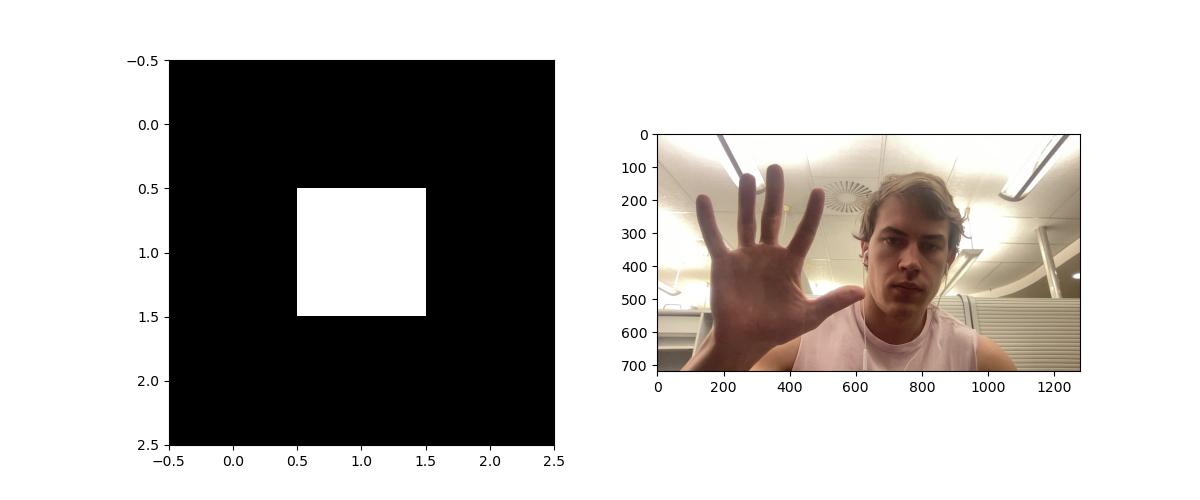
\includegraphics[width=0.9\linewidth]{figures/kernel_identity.png}
    \caption{Input image to various kernel functions}
    \label{fig:kernel_identity}
\end{figure}

\begin{figure}[h]
    \centering
    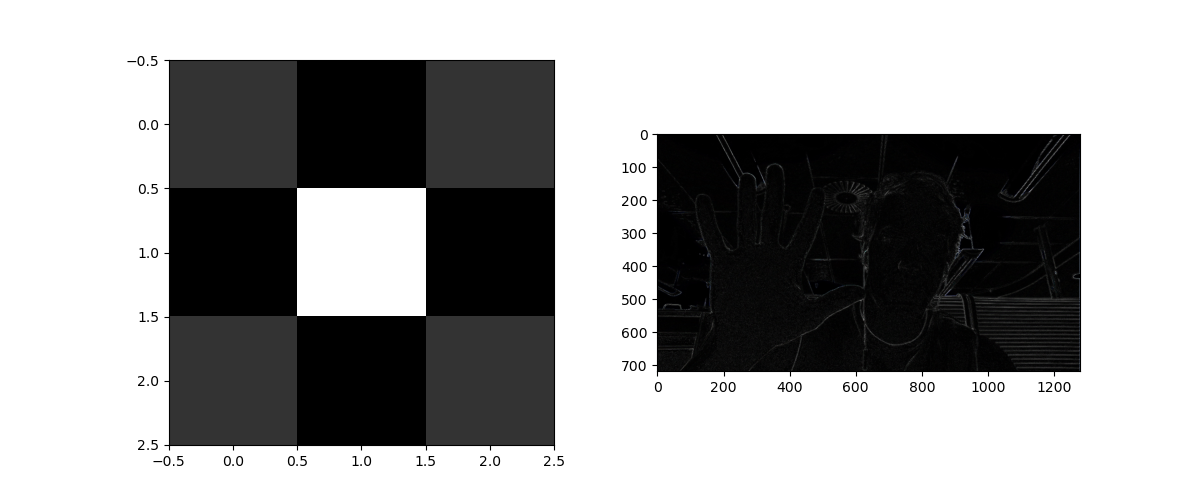
\includegraphics[width=0.9\linewidth]{figures/kernel_edge_detection_1.png}
    \caption{Output of the edge detection 1 kernel function}
    \label{fig:kernel_edge_detection_1}
\end{figure}

\begin{figure}[h]
    \centering
    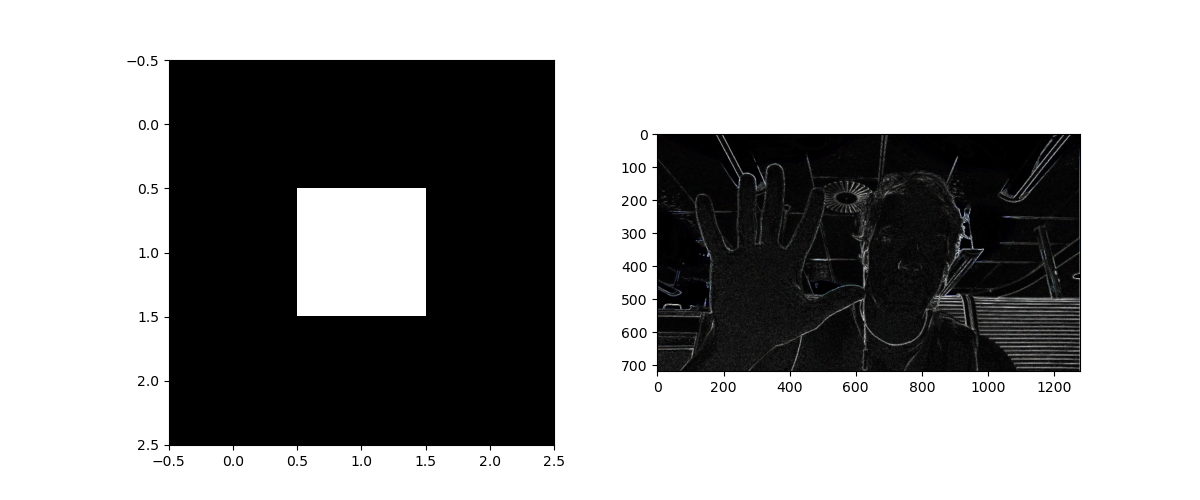
\includegraphics[width=0.9\linewidth]{figures/kernel_edge_detection_2.png}
    \caption{Output of the edge detection 2 kernel function}
    \label{fig:kernel_edge_detection_2}
\end{figure}

\begin{figure}[h]
    \centering
    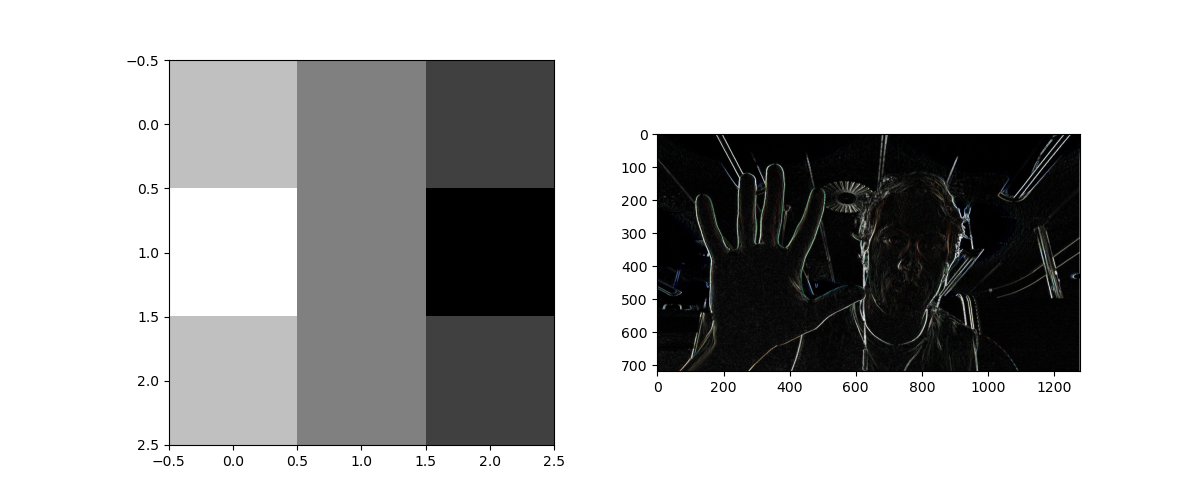
\includegraphics[width=0.9\linewidth]{figures/kernel_left_sobel.png}
    \caption{Output of the left sobel kernel function}
    \label{fig:kernel_left_sobel}
\end{figure}

\begin{figure}[h]
    \centering
    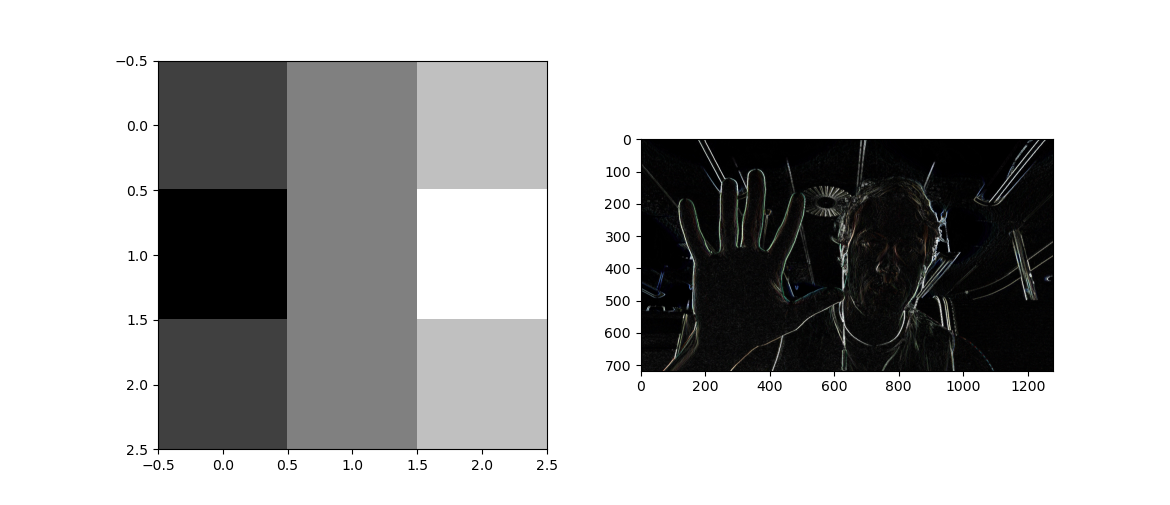
\includegraphics[width=0.9\linewidth]{figures/kernel_right_sobel.png}
    \caption{Output of the right sobel kernel function}
    \label{fig:kernel_right_sobel}
\end{figure}

\section[2022/05/31]{Tuesday, 31 May 2022}

\subsection{OpenGL Cube Experimentation}

The aim of this session is to illustrate the work done in the previous week on the three-dimensional rendering of a cube in a video stream. \\

In order to properly create an augmented reality application the virtual object must be rendered continuously alongside a changing input video stream with different transformations and perspectives in order to create augmented reality. The rendering of this virtual object will be accomplished using a library. OpenGL is the de-facto standard for rendering three-dimensional scenes on modern hardware and it possesses a computationally efficient Python wrapper API. This API was used to render a basic cube as seen in \FigRef{fig:OpenGL_cube}.\\

\begin{figure}[h]
    \centering
    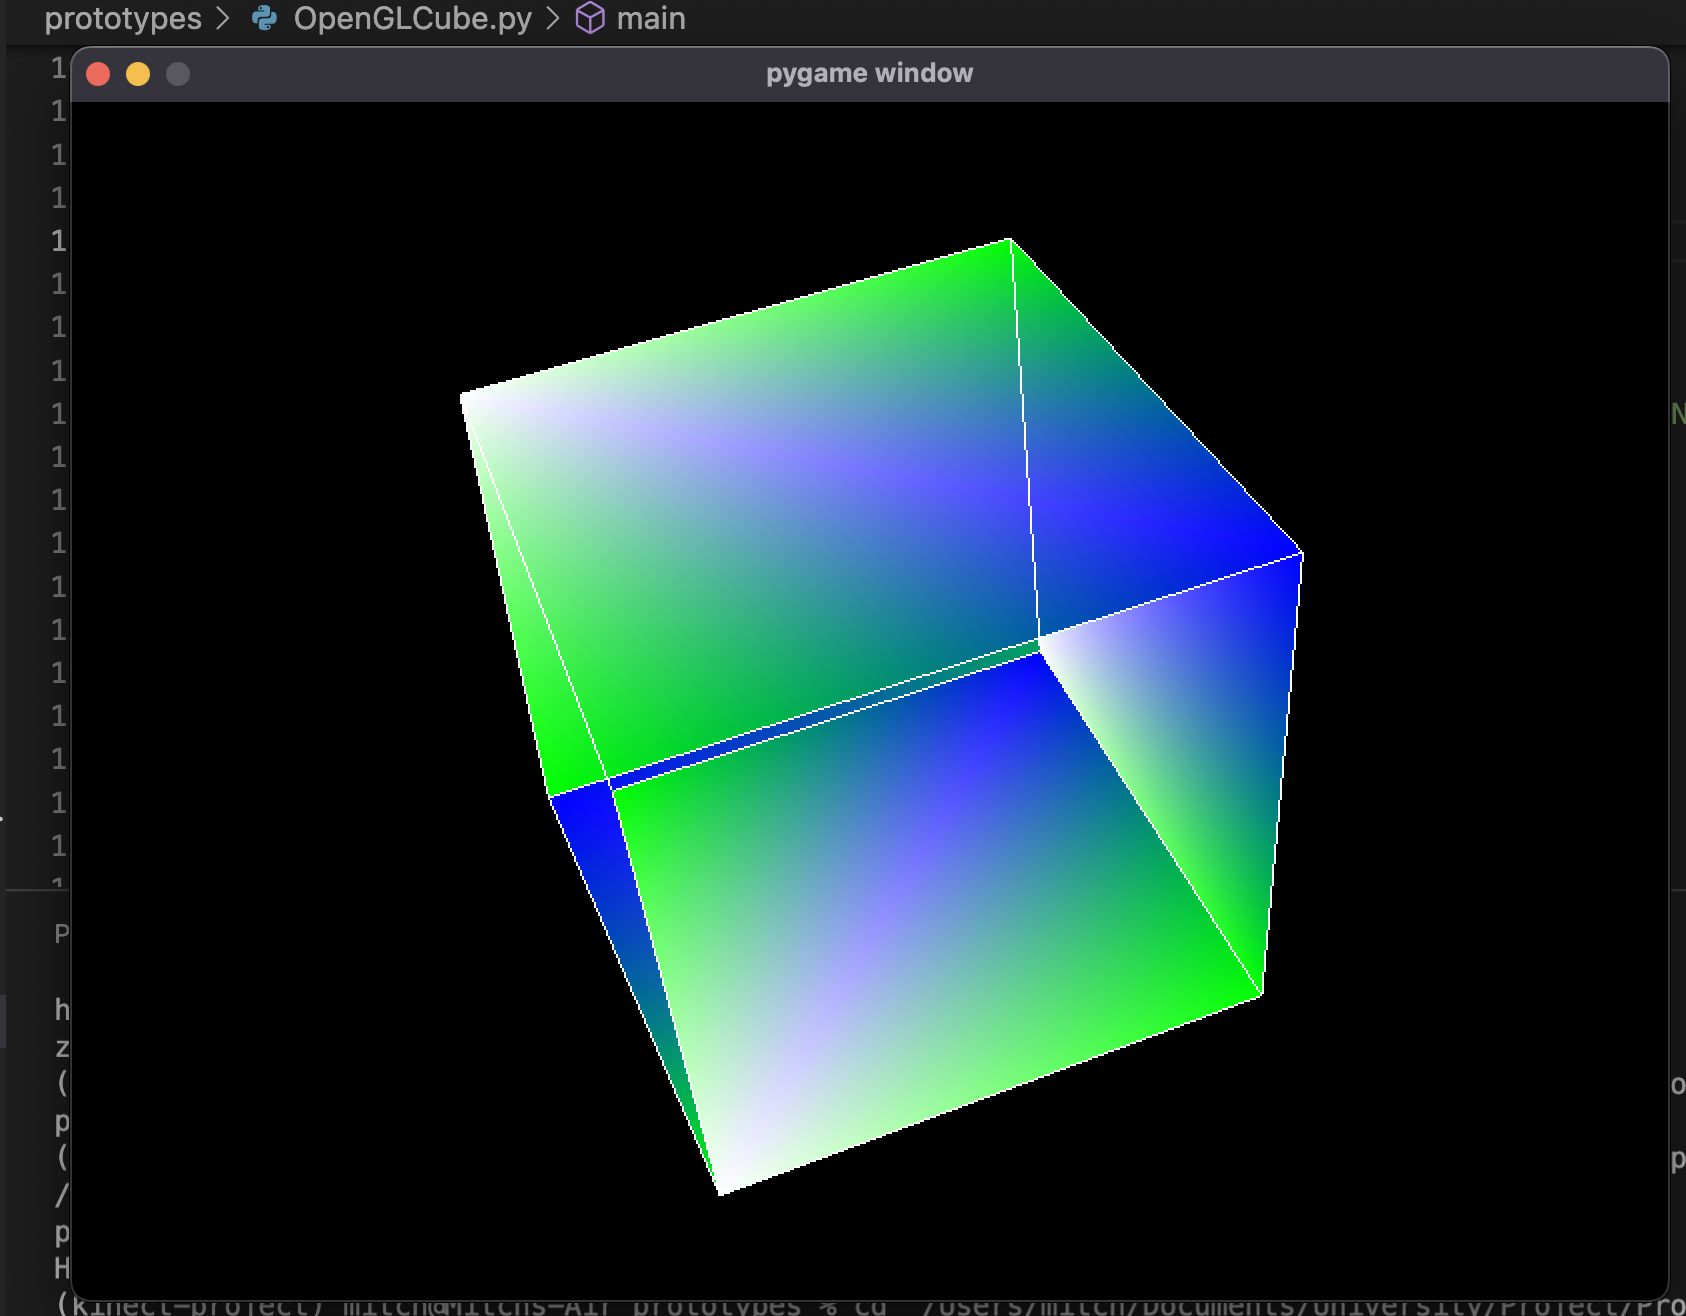
\includegraphics[width=0.6\linewidth]{figures/OpenGL_cube.png}
    \caption{Output of the OpenGL cube rendering program}
    \label{fig:OpenGL_cube}
\end{figure}

OpenGL utilizes a series of vertices and lines between these vertices in order to draw three-dimensional shapes. The cube obviously consists of these primitive shapes but the background too is merely a giant rectangle that stretches the length of the screen and has mapped to it the texture of the input video feed - broadcast to it from a webcam. This effect is visible in \FigRef{fig:OpenGL_cube1.png}. Further work needs to be done to investigate the rotation of objects in the OpenGL application as well as perspective changes needed to make the object appear smaller and larger at different times.\\

\begin{figure}[h]
    \centering
    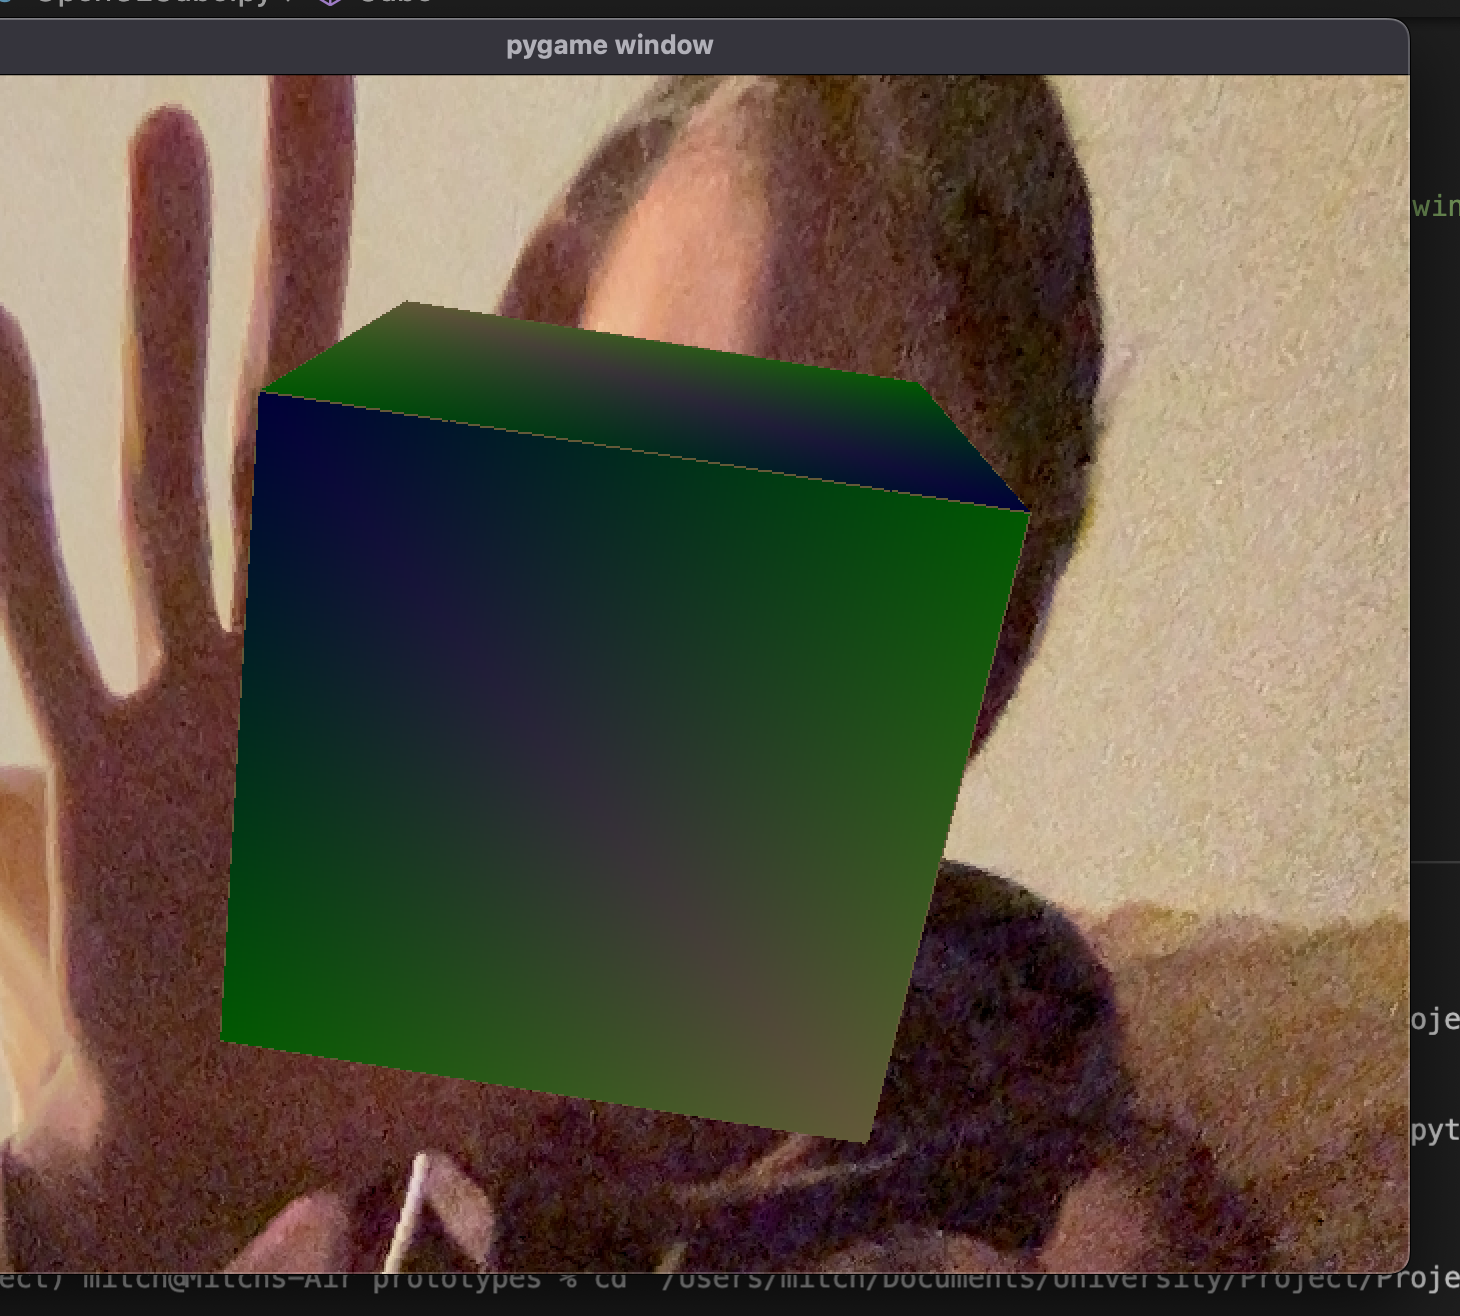
\includegraphics[width=0.6\linewidth]{figures/OpenGL_cube1.png}
    \caption{Output of the OpenGL cube rendering program overlaid on a video input feed}
    \label{fig:OpenGL_cube1.png}
\end{figure}